\documentclass[../main.tex]{subfiles}

\begin{document}

\section{Design}

%Indledning af design-afsnittet
\begin{flushleft} 
Intro tekst
\end{flushleft}


%Indledning til GRASP-principper
\subsection{GRASP (!Indsat kopi fra CDIO-2!)}
\TODO[Må vi kopiere denne del fra CDIO-2?]
\begin{flushleft}
Vi vil benytte GRASP principperne til at designe vores diagrammer, således at software-klasserne har et veldefineret og afgrænset ansvar som understøtter reusability. \newline
\newline
De følgende GRASP principper forklares og argumenteres for under designklassediagrammet:
\begin{itemize}
    \item Creator: Ansvar for objektskabelse
    \item Information Expert: Ansvar for tildeling af ansvar til objekter
    \item Low Coupling: Ansvar for lav afhængighed/associationer mellem klasserne
    \item High Cohesion: Ansvar for høj samhørighed mellem klasserne
    \item Controller: Ansvar for input til systemet
\end{itemize}
\end{flushleft}


%Designklassediagram
\subsection{Designklassediagram (!Indsat kopi fra CDIO-2!)}
\TODO[Må vi kopiere denne del fra CDIO-2?]
\begin{flushleft}
Et designklassediagram laves på baggrund af GRASP-principperne samt tidligere analytiske arbejde med særligt udgangspunkt i  vores domænemodel (Figur \ref{fig:domain}), som indeholder concepter af klasser. I designklassediagrammet arbejder vi med software-klasser, som skal implementeres i systemet. Her har software-klasserne mere konkrete beskrivelser end domænemodellen. Derfor er der bl.a. beskrevet attributter, tilhørende metoder og relationer mellem klasserne. Designklassediagrammet arbejdes dermed også videre på i implementationsfasen, da der vil opstå ændringer undervejs. Understående diagram er vores endelige dokumenterede designklassediagram for systemet:
\end{flushleft}

%Designklassediagram
\begin{figure}[H]
    \centering
    \rotatebox{270}{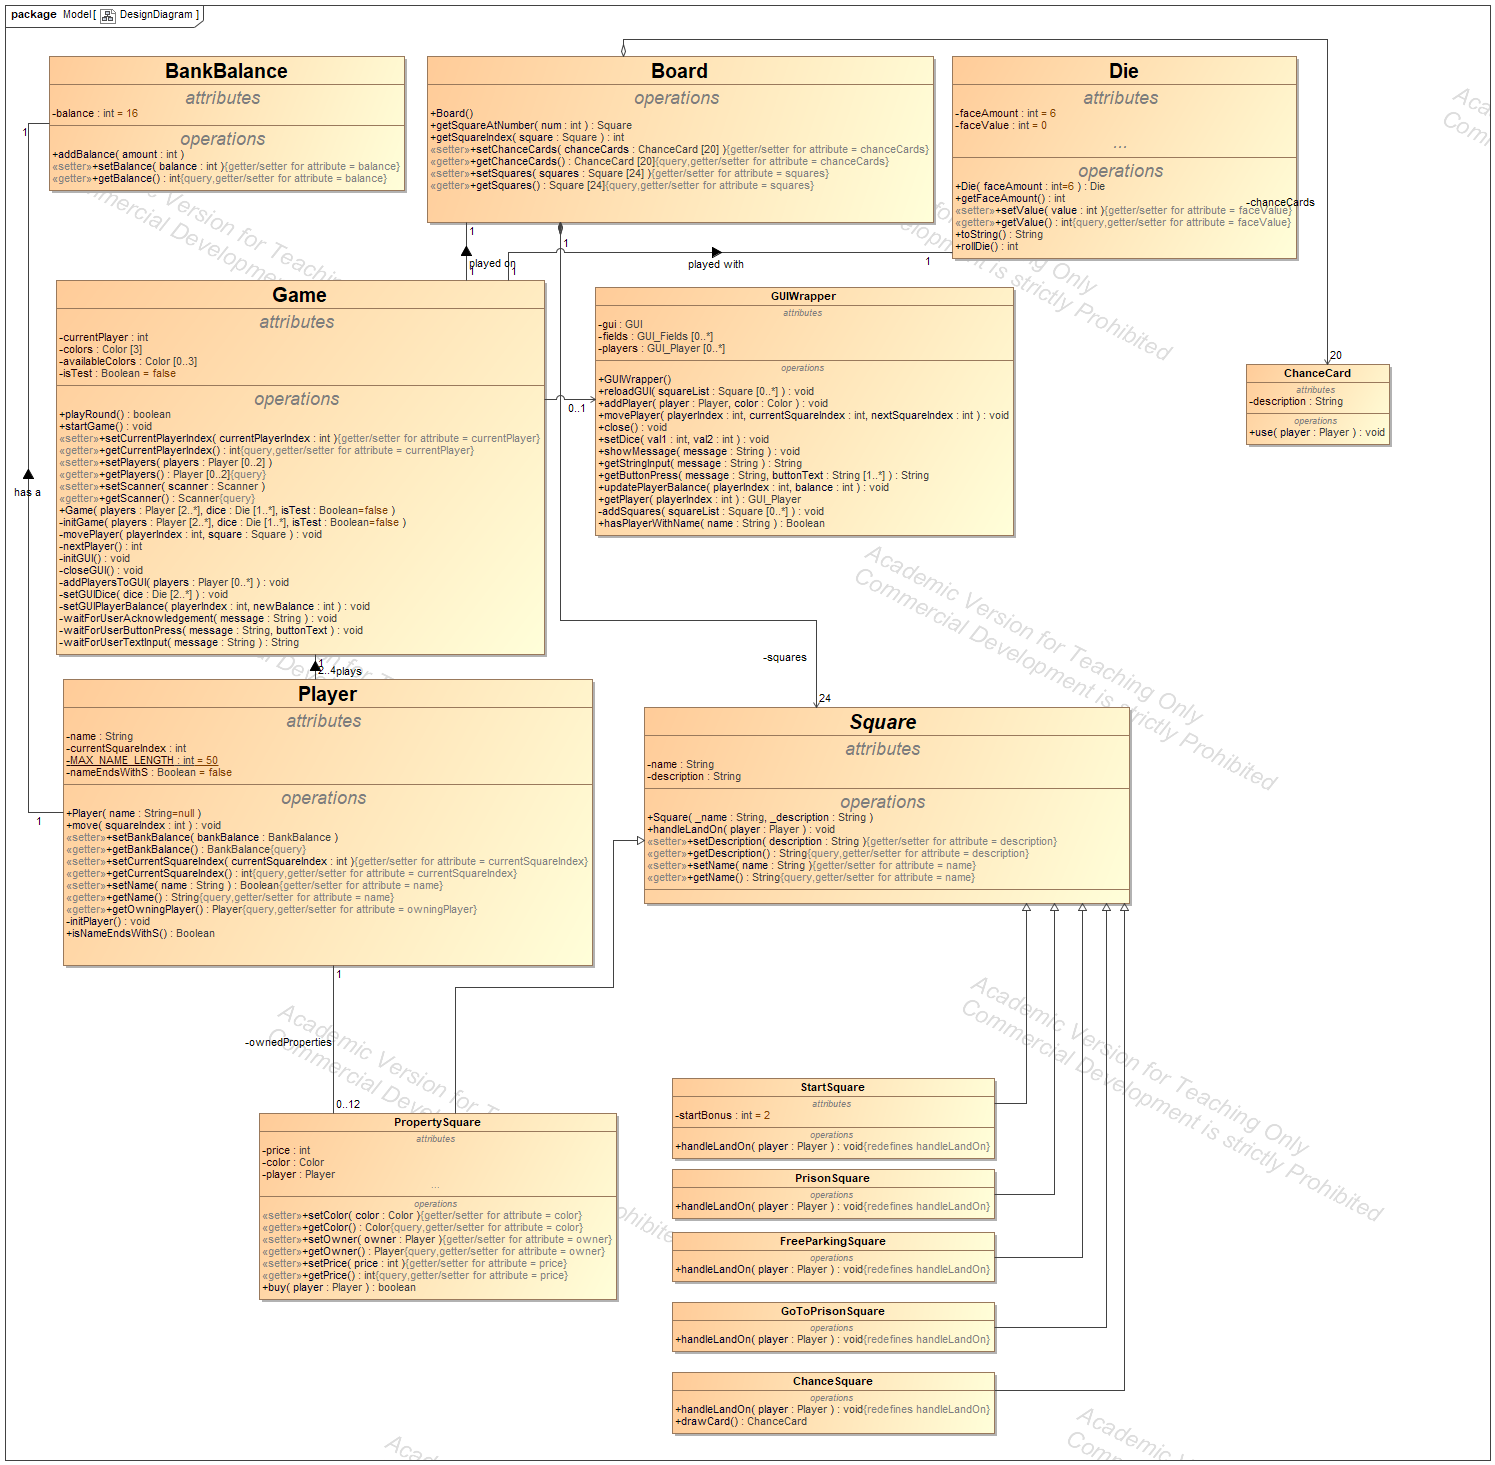
\includegraphics[width=0.92\textheight]{figures/designklassediagram.png}}
    \caption{Designklassediagram}
    
    \label{fig:designclass}
\end{figure}


% GRASP-principper i designklassediagram
\subsubsection{GRASP principper for designklassediagram}
\begin{flushleft}
\begin{itemize}
    \item Creator: 
    \begin{itemize}
        \item  
        \item  
    \end{itemize}
    \item Information Expert:
    \begin{itemize}
        \item  
        \item 
    \end{itemize}
    \item Low Coupling:
    \begin{itemize}
        \item
        \item
    \end{itemize}
    \item High Cohesion:
    \begin{itemize}
        \item
        \item
    \end{itemize}
    \item Controller: 
    \begin{itemize}
        \item 
    \end{itemize}
\end{itemize}
\end{flushleft}


% Sekvensdiagram
\subsection{Sekvensdiagram }
\begin{flushleft}
Intro sekvensdiagram
\end{flushleft}

%Sekvensdiagram for Game og Die?
\subsubsection{Indsæt klasser}
\begin{figure}[H]
    \centering
   {\includegraphics[width=0.5\textheight]{figures/}}
    %\includegraphics[width=0.6\linewidth]{figures/DesignClassDiagram.jpg}
    \caption{Sekvensdiagram over ...}
    \label{fig:sekvensdia1}
\end{figure}


%Pakkediagram? (Måske)
\subsection{Pakkediagram (Måske) }


\end{document}
